\documentclass[../../D1.tex]{subfiles}

\begin{document}

%The explosion of Deep Neural Network applications in recent years has prompted the production of a wave of specialised hardware architectures to improve the efficiency and compute of these kinds of workloads. The mainstay of this form of processing has been until recently been dominated by GPUs.\\


\subsubsection{Memory Allocation}\label{sec:MemAlloc}
\begin{figure}[H]
    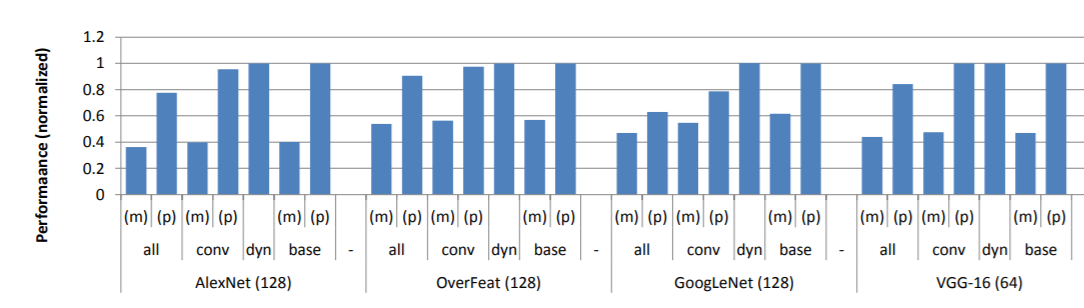
\includegraphics[width=1\textwidth]{vDNNperf.png} 
    \caption{vDNN performance, showing the throughput using various memory allocation strategies. \\ \textbf{(Adopted figure from~\autocite{rhuVDNNVirtualizedDeep2016})}}
    \label{fig:vDNNperf}   
\end{figure}

While designed specifically for training networks that would otherwise be to large for a GPU, the memory manager vDNN proposed by Rhu et al~\autocite{rhuVDNNVirtualizedDeep2016}~does provide some insight into the importance of memory locality to neural network throughput.
Fig.~\ref{fig:vDNNperf}~summarizes the performance of neural networks using vDNN to manage memory compared to a baseline memory management policy ($base$). The vDNN policies include: static policies (denoted as $all$ and $conv$) and a dynamic policy ($dyn$).
$base$ simply loads the full model into the GPU memory, consequently providing optimal memory locality. $all$ refers to a policy of moving all $X$s out of GPU memory, and $conv$ only offloads $X$s from convolutional layers, $X$s are the input matrices to each layer, denoted by the red arrows in Fig.~\ref{fig:memAllocInf}.
Each of $base$, $conv$ and $all$ are evaluated using two distinct convolutional algorithms - memory-optimal ($m$) and performance-optimal ($p$).
Finally the $dyn$ allocation policy chooses ($m$) and ($p$) dynamically at runtime.

Observing the results in Fig.~\ref{fig:vDNNperf}~where performance is characterized by latency during feature extraction layers; a significant performance loss is evident in the $all$ policy compared to baseline, this loss is caused because no effort is made to optimise the location of network parameters in memory.
In this example the memory allocations are being measured between memory in the GPU (VRAM) and host memory (DRAM) accessed via the PCI lanes. This does show how important the latency in memory access can be crucial for model throughput.

\begin{figure}[H]
    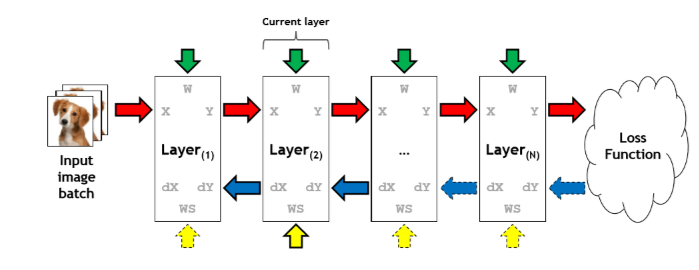
\includegraphics[width=1\textwidth]{MemoryAlloc.png} 
    \caption{Memory allocations required for linear networks. All green ($W$) and red ($X$) arrows are allocated during inference, the blue and yellow arrows are allocated during training.\\ \textbf{(Adopted figure from~\autocite{rhuVDNNVirtualizedDeep2016})}}
    \label{fig:memAllocInf}   
\end{figure}


\subsubsection{Memory Access}

A significant portion of DNN computation is matrix-vector multiplication, ideally weight reuse techniques can speed up these operations.
However some DNNs feature FC layers with more than a hundred million weights (Fig.~\ref{fig:CNNcomplexity}), memory bandwidth here can be an issue since loading these weights can be a significant bottleneck~\autocite{qiuGoingDeeperEmbedded2016}. 
As observed in Section~\ref{sec:MemAlloc} this indicates that compression (Section~\ref{subsec:compressionTypes}) techniques could help alliviate this bottleneck by making parameters avaliable for cache reuse.

\begin{figure}[H]
    \begin{center}
        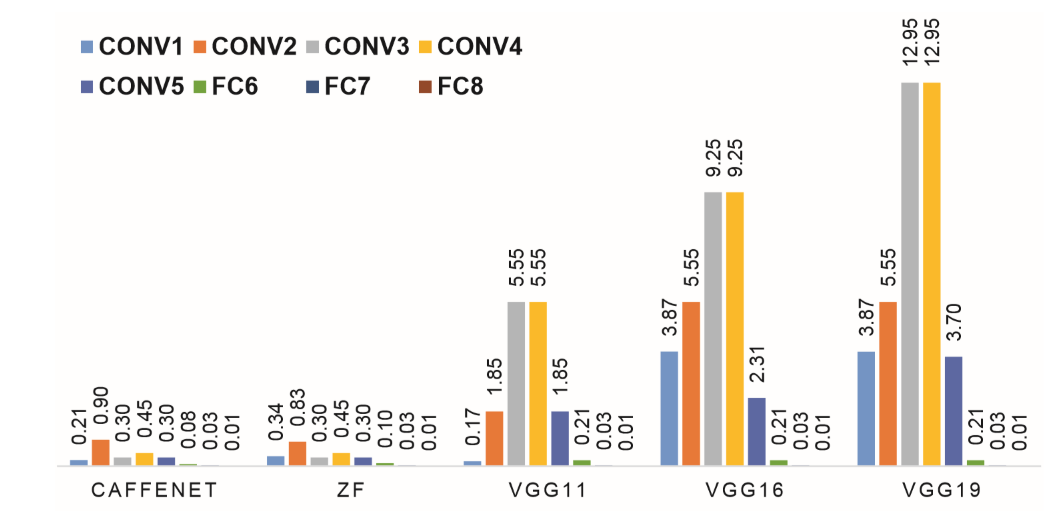
\includegraphics[width=0.7\textwidth]{OperationDemand.png} 
    \end{center}
    
    \caption{Operations demanded in different layers (GOP)\\ \textbf{(Adopted figure from~\autocite{qiuGoingDeeperEmbedded2016})}}
    \label{fig:CNNcomplexity}   
\end{figure}

Often modern networks are so large and complex there can still be an insufficient cache capacity for the full network parameters even when using modern compression techniques such as described in~\autocite{hanDeepCompressionCompressing2016}, in a follow up paper Han et al.~\autocite{hanEIEEfficientInference2016} discuss this case where memory accesses occur for every operation because the codebook (from a pruned and then quantised network) cannot be reused properly.
This paper proposes EIE (an \acrshort{fpga} inference engine for compressed networks) also shows that while compression does reduce the total number of operations, and a tangible speedup can be observed in the FC layers see Fig.~\ref{fig:wallClockEIE}, this technique when applied to convolutional layers has some issues.


Han et al~\autocite{hanEIEEfficientInference2016} provide an elegant description of a technique for exploiting the sparity of activations by storing an encoded sparse weight matrix in a variant of compressed sparse column format~\autocite{vuducAutomaticPerformanceTuning}, however implementing this is problematic (particularly in convolutional layers) due to the irregular memory access patterns, lack of library and kernel level support for this style of sparse matrix (as discussed in Section~\ref{sec:Pruning}). 
It should also be noted that Fig.~\ref{fig:wallClockEIE} is comparing general purpose compute hardware with a custom built \acrshort{fpga}, so the speedup while impressive would be more appropriate compared to other purpose built \acrshort{fpga}s, however the most pertinent part of this Figure is the single batch size \acrshort{fc} layer comparison between dense and sparse matrices.


\begin{figure}[H]
    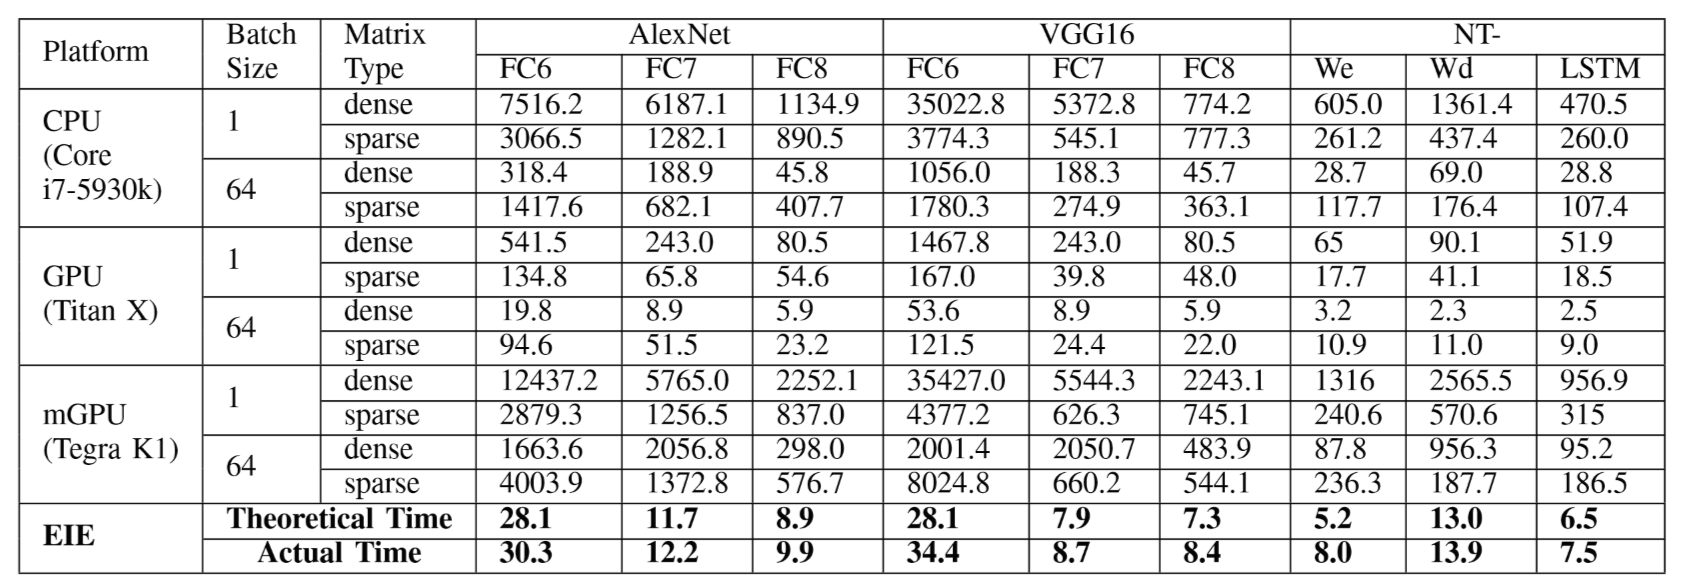
\includegraphics[width=1\textwidth]{wallClockEIE.png} 
    \caption{Wall clock time ($\mu$) comparison for sparse and dense matrices in FC layers between CPU, GPU, mGPU and EIE (an FPGA custom accelerator)\\ \textbf{(Adopted figure from~\autocite{hanEIEEfficientInference2016})}}
    \label{fig:wallClockEIE}   
\end{figure}


\end{document}